% Thesis Figure 5.4: macro-F1 for the five evaluated graph and hypergraph models.
% T-032 replaces five values printed in the source publication with the author's
% corrected five-run mean records. Keep these values aligned with
% Tables 5.1 and 5.2 in content/hgann-mal.tex.
\documentclass[border=1pt]{standalone}
\usepackage[T1]{fontenc}
\usepackage{tgheros}
\renewcommand{\familydefault}{\sfdefault}
\usepackage{tikz}
\usetikzlibrary{calc}

\definecolor{tumblue}{HTML}{0065BD}
\definecolor{tumblueii}{HTML}{64A0C8}
\definecolor{tumblueiii}{HTML}{98C6EA}
\definecolor{tumgrey}{HTML}{808080}
\definecolor{tumgreylight}{HTML}{CCCCCC}
\definecolor{tumgreydark}{HTML}{333333}

\newcommand{\labelfont}{\fontsize{6.2}{7.1}\selectfont}
\newcommand{\valuefont}{\fontsize{6.0}{6.9}\selectfont\bfseries}
\newcommand{\axisfont}{\fontsize{6.0}{6.9}\selectfont}
\newcommand{\titlefont}{\fontsize{7.6}{8.7}\selectfont\bfseries}
\newcommand{\gainfont}{\fontsize{5.8}{6.7}\selectfont}

% A score of 80 lies on the panel baseline. Each percentage point occupies 1.5 mm.
\newcommand{\scorey}[2]{#1+(#2-80)*1.5}
\newcommand{\scorebar}[4]{%
  \pgfmathsetmacro{\barheight}{(#3-80)*1.5}%
  \filldraw[fill=#4,draw=#4!85!black,line width=0.25pt]
    (#2-2.15,#1) rectangle (#2+2.15,#1+\barheight);
  \node[above,inner sep=0.8pt] at (#2,#1+\barheight) {\valuefont #3};
}

\newcommand{\panelgrid}[2]{%
  \foreach \v in {80,85,90,95,100}{%
    \pgfmathsetmacro{\yy}{#2+(\v-80)*1.5}%
    \draw[tumgreylight,line width=0.3pt] (12,\yy) -- (140,\yy);
    \node[left,text=tumgrey,inner sep=1pt] at (11.2,\yy) {\axisfont \v};
  }%
  \node[anchor=west,inner sep=0pt] at (1,#2+34.2) {\titlefont #1};
}

\newcommand{\legenditem}[3]{%
  \filldraw[fill=#3,draw=#3!85!black,line width=0.25pt]
    (#1,122.0) rectangle (#1+3.2,125.2);
  \node[anchor=west,inner sep=0pt] at (#1+4.4,123.6) {\labelfont #2};
}

\begin{document}
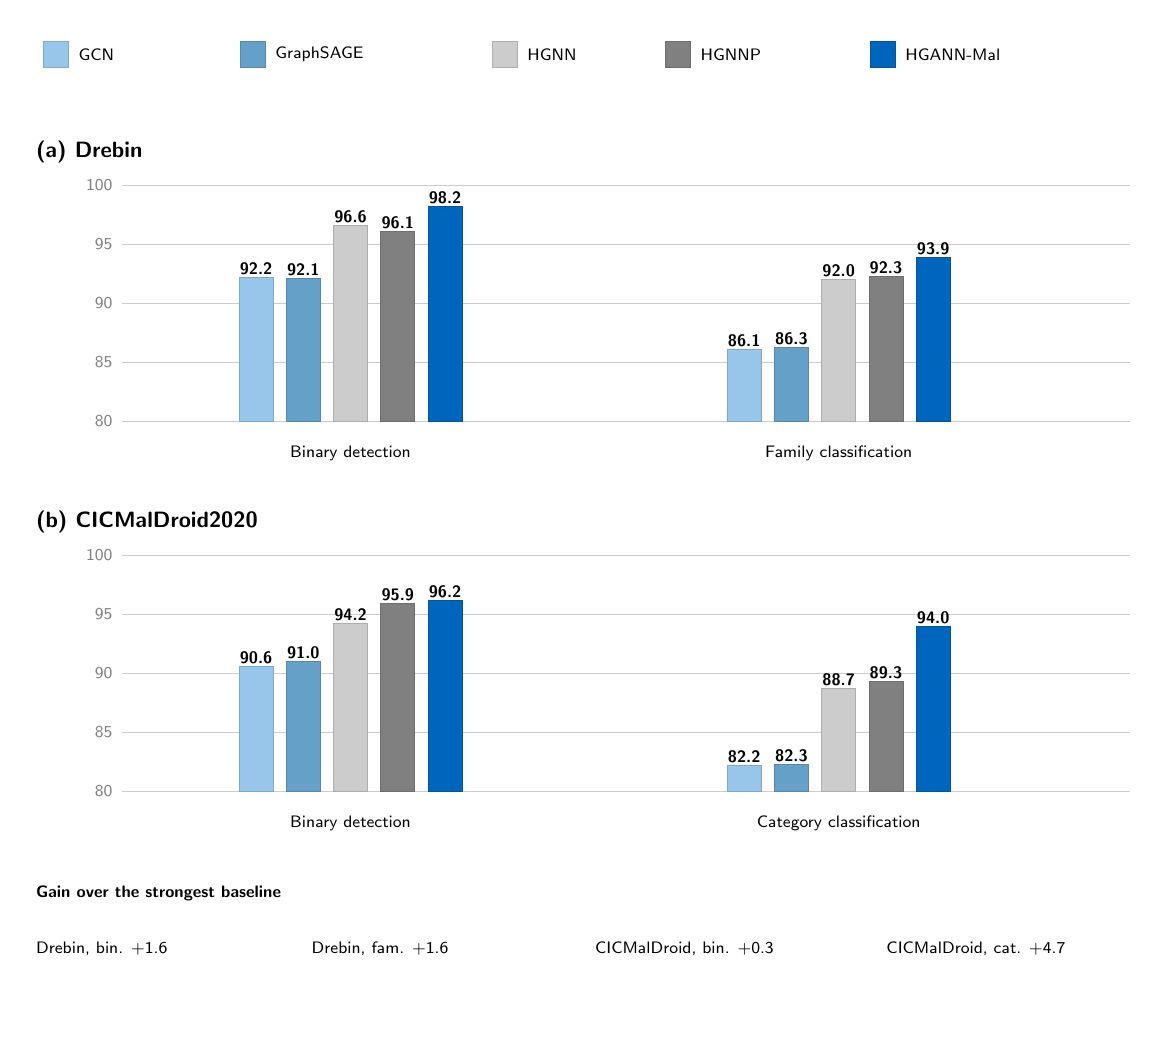
\begin{tikzpicture}[x=1mm,y=1mm]
  \useasboundingbox (0,0) rectangle (141.6,127);

  \legenditem{2}{GCN}{tumblueiii}
  \legenditem{27}{GraphSAGE}{tumblueii}
  \legenditem{59}{HGNN}{tumgreylight}
  \legenditem{81}{HGNNP}{tumgrey}
  \legenditem{107}{HGANN-Mal}{tumblue}

  % Drebin panel.
  \panelgrid{(a) Drebin}{77}
  \scorebar{77}{29}{92.2}{tumblueiii}
  \scorebar{77}{35}{92.1}{tumblueii}
  \scorebar{77}{41}{96.6}{tumgreylight}
  \scorebar{77}{47}{96.1}{tumgrey}
  \scorebar{77}{53}{98.2}{tumblue}
  \scorebar{77}{91}{86.1}{tumblueiii}
  \scorebar{77}{97}{86.3}{tumblueii}
  \scorebar{77}{103}{92.0}{tumgreylight}
  \scorebar{77}{109}{92.3}{tumgrey}
  \scorebar{77}{115}{93.9}{tumblue}
  \node at (41,73.0) {\labelfont Binary detection};
  \node at (103,73.0) {\labelfont Family classification};

  % CICMalDroid panel.
  \panelgrid{(b) CICMalDroid2020}{30}
  \scorebar{30}{29}{90.6}{tumblueiii}
  \scorebar{30}{35}{91.0}{tumblueii}
  \scorebar{30}{41}{94.2}{tumgreylight}
  \scorebar{30}{47}{95.9}{tumgrey}
  \scorebar{30}{53}{96.2}{tumblue}
  \scorebar{30}{91}{82.2}{tumblueiii}
  \scorebar{30}{97}{82.3}{tumblueii}
  \scorebar{30}{103}{88.7}{tumgreylight}
  \scorebar{30}{109}{89.3}{tumgrey}
  \scorebar{30}{115}{94.0}{tumblue}
  \node at (41,26.0) {\labelfont Binary detection};
  \node at (103,26.0) {\labelfont Category classification};

  \node[anchor=west,inner sep=0pt] at (1,17.0)
    {\gainfont\bfseries Gain over the strongest baseline};
  \node[anchor=west,inner sep=0pt] at (1,10.0) {\gainfont Drebin, bin. +1.6};
  \node[anchor=west,inner sep=0pt] at (36,10.0) {\gainfont Drebin, fam. +1.6};
  \node[anchor=west,inner sep=0pt] at (72,10.0) {\gainfont CICMalDroid, bin. +0.3};
  \node[anchor=west,inner sep=0pt] at (109,10.0) {\gainfont CICMalDroid, cat. +4.7};
\end{tikzpicture}
\end{document}
